\begin{figure}[h!]
   \centering
   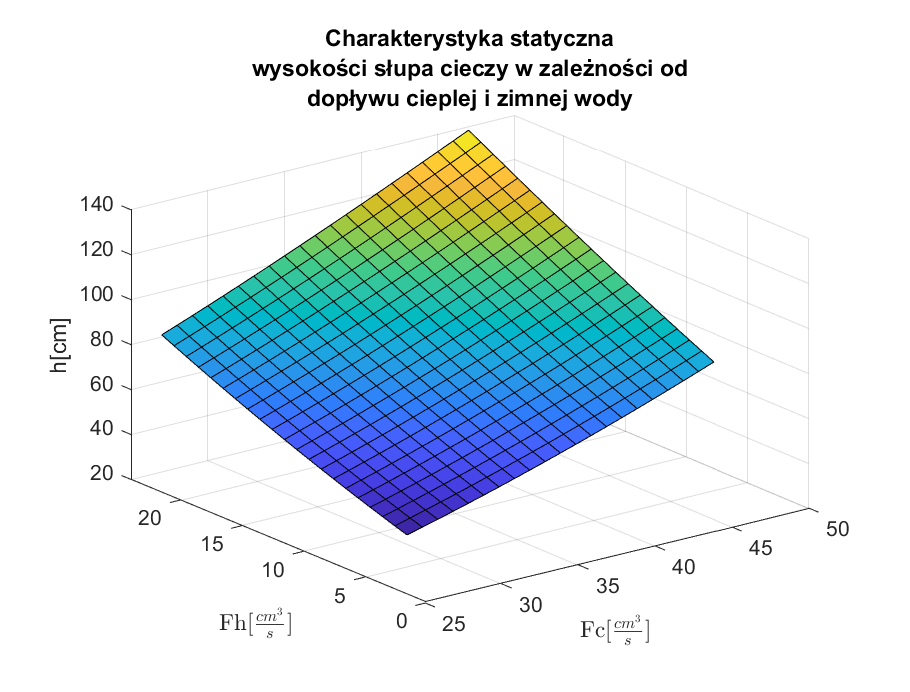
\includegraphics{img/static/staticV.eps}
   \caption{Charakterystyka statyczna pojemności zbiornika}
   \label{fig:staticV}
\end{figure}
            
\begin{figure}[h!]
   \centering
   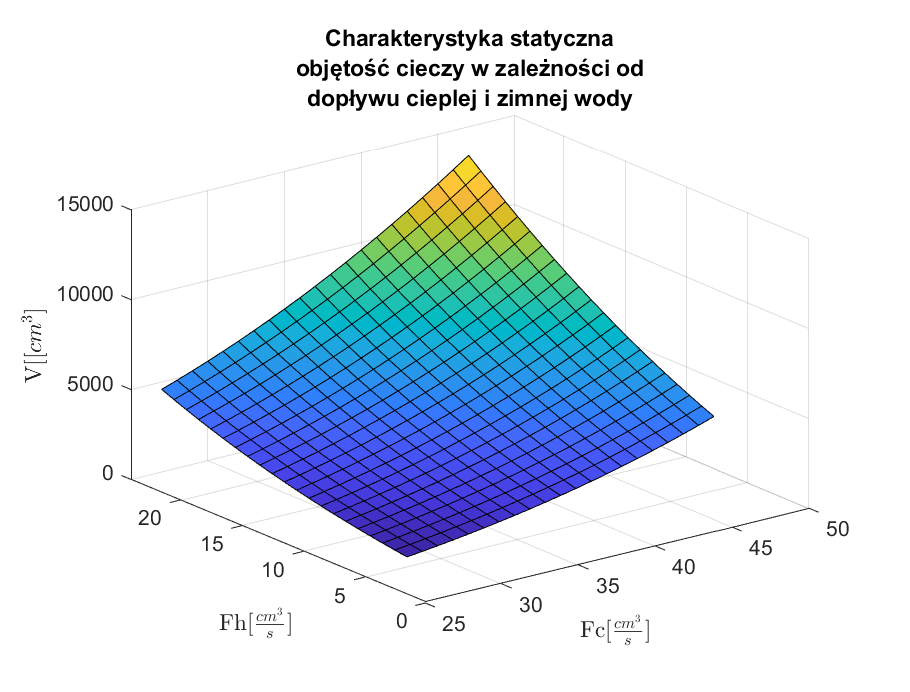
\includegraphics{img/static/staticH.eps}
   \caption{Charakterystyka statyczna wysokości słupa cieczy w zbiorniku}
   \label{fig:staticH}
\end{figure}
            
\begin{figure}[h!]
   \centering
   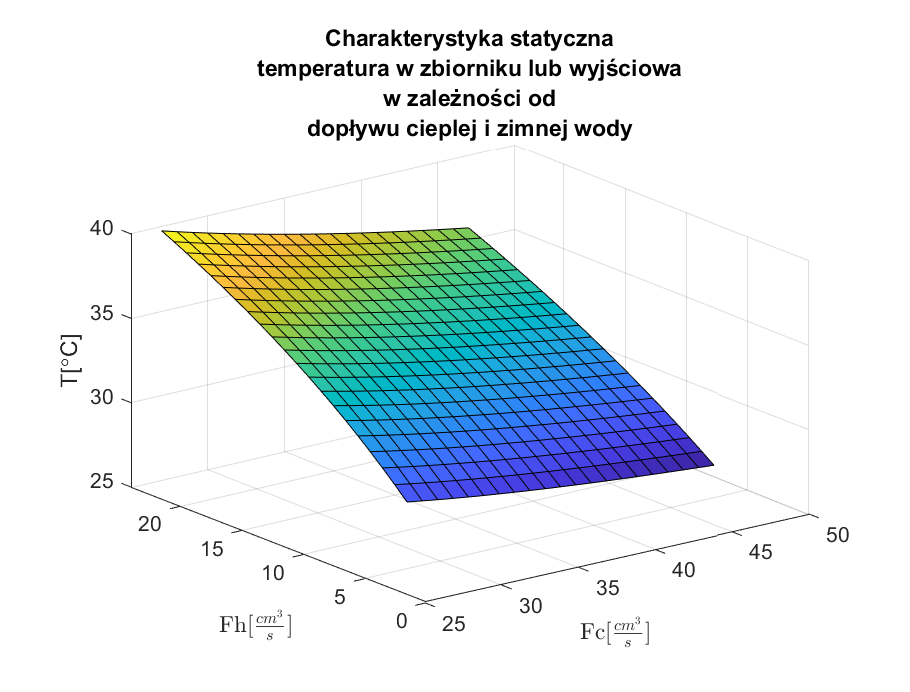
\includegraphics{img/static/staticT.eps}
   \caption{Charakterystyka statyczna temperatury cieczy w zbiorniku, czy na wyjściu zbiornika}
   \label{fig:staticT}
\end{figure}
            
